\section{Hilbert Spaces}
\label{section:hilbert-spaces}

\begin{quote}
  "Hilbert spaces are the means by which the ordinary experience of Euclidian concepts can be extended meaningfully into the idealized constructions of more complex math." \citep{bernkopf2008schmidt}
\end{quote}

Originally, conceptual spaces \citep{gardenfors2004conceptual} were formalized by using Euclidian or Manhattan distances to measure similarity in conceptual spaces modeled in constrained Cartesian-like space. Though this is useful in building an intuition as to how conceptual spaces operate in practice, it can be limiting in the description of relations between objects and the space itself.  In order to allow for more flexibility in this regard, we need a more general notion of a space than a finite-dimensional Euclidian space.  The generalization employed here is that of Hilbert spaces \citep{kennedy2013hilbert}, which generalizes the pedestrian finite-dimensional Euclidian space to infinite-dimensional spaces with arbitrary geometry.

\subsection{Complete Inner Product Space} 
\label{subsection:complete-inner-product-space}

A Hilbert space is defined as a complete inner product space.  That is, a Hilbert space is a vector space equipped with an inner product $\innerproduct$, but is also complete: the space is big enough to include the norm of converging sequences.  In the case of an infinite-dimensional Hilbert space, this completeness criterion cannot be taken for granted, but in the finite-dimensional case, the space is always complete.  The inner product of a Hilbert space induces a norm $\|f\| = \langle f, f \rangle^{1/2}$, which allows us to talk about distances between vectors, something that we require in a generalized formalism of conceptual spaces.

What makes Hilbert spaces powerful is the ability to represent a function as a point in the space.  With the aid of the inner product, one can produce an (infinite) orthonormal sequence $\orthseq$ for the Hilbert space.  By decomposing any function $f$ into its Fourier series (equation \ref{equation:fourier-series}) on that sequence, we can recover a corresponding coefficient $\langle f, \varphi_n \rangle$ corresponding to each element of the orthonormal sequence.

\begin{equation} 
  \label{equation:fourier-series}
  f = \sum_{n=0}^\infty \langle f, \varphi_n \rangle \varphi_n
\end{equation}

By arranging each of these coefficients into a vector with dimensions $\varphi_n$, the function can be represented as a point in the Hilbert space. If that space is finite, we can equivalently represent a point $x$ in the Hilbert space as an array of complex numbers, $x \in \mathbb{C}^n$ where $n$ is the number of dimensions.

\subsection{Application to Conceptual Spaces}
\label{subsection:application-conceptual-spaces}

Now, by defining a conceptual space formally in terms of a Hilbert space, we see that the geometry of the conceptual space can be fully defined by the inner product of the Hilbert space.  This has two consequences.  First, since for a given function, the Fourier series decomposition generates a vector representation, any number of different vectors can be produced from the same function for each inner product.  This means that a given object can be represented in any number of conceptual spaces defined by their inner product.

Conversely, since it can be proven that all Hilbert spaces of the same number of dimensions are isomorphic \citep{kennedy2013hilbert}, given a vector, we can then choose an inner product to determine its representation.  In this way, each inner product imposes a geometry that allows for different perspectives of the same "raw" data.  By analogy, in figure \ref{figure:cartesian-radial} we see that coordinates represented on $(x, y)$ in a 2D Cartesian space have a different meaning and location than if they are represented on $(r, \theta)$ in a 2D radial space.  This allows for complete flexibility in representation, as an object can be placed in a conceptual space simply by interpreting its vector representation according to the inner product of that space. \citep{wiggins2018creativity}

\begin{figure}
  \centering
  \begin{subfigure}{0.45\linewidth}
    \def\svgwidth{\linewidth}
    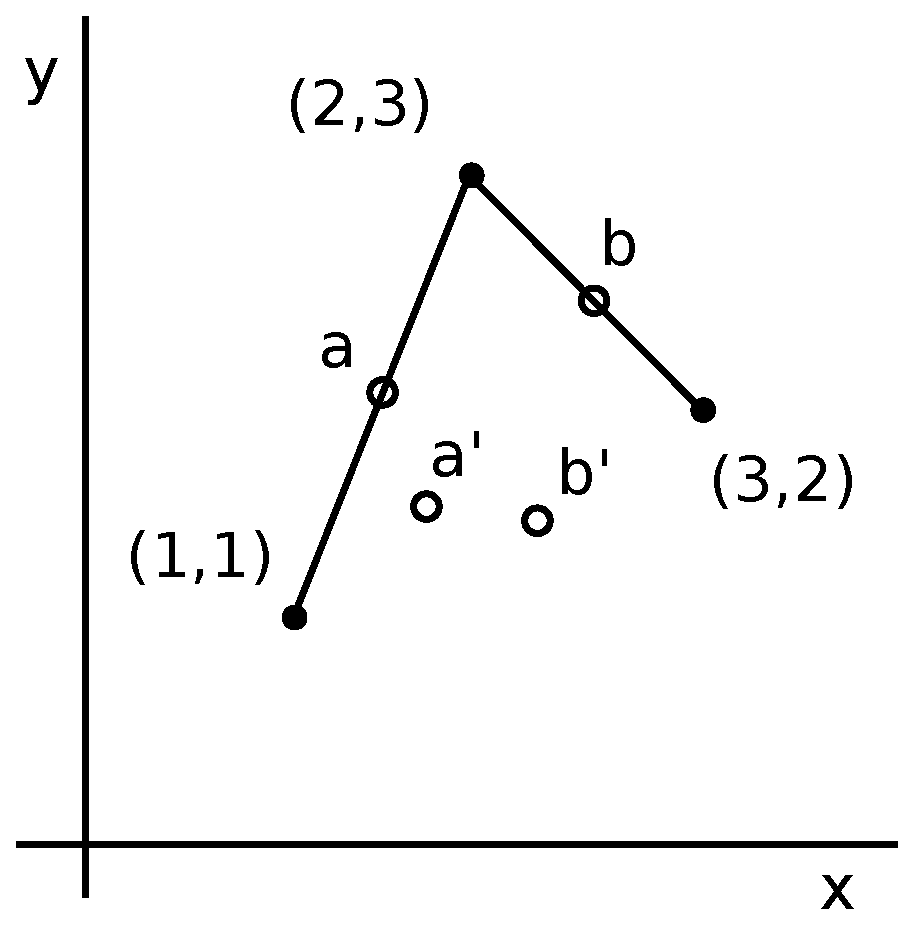
\includegraphics[width=\linewidth]{fig/interpolation-cartesian.eps}
    \caption{Cartesian Trajectory}
  \end{subfigure}
  \begin{subfigure}{0.45\linewidth}
    \def\svgwidth{\linewidth}
    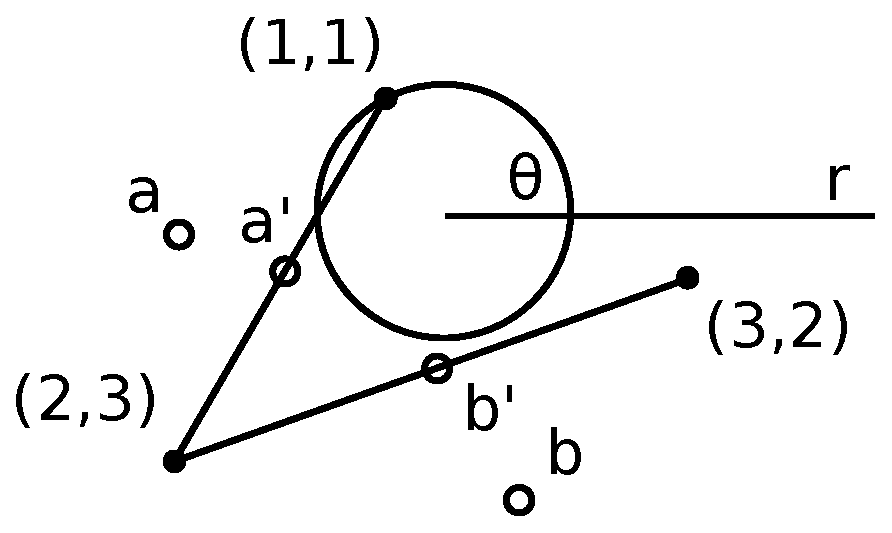
\includegraphics[width=\linewidth]{fig/interpolation-radial.eps}
    \caption{Radial Trajectory}
  \end{subfigure}
  \caption{Effect of the inner product on spatial geometry}
  \label{figure:cartesian-radial}
\end{figure}


